\documentclass[11pt]{article}
\usepackage[margin=1in]{geometry}\usepackage{booktabs,tabularx,hyperref,graphicx,amsmath}
\title{VERA Evidence Feedback: Novelty and Feasibility Gate}\author{Research update for Shrid Pant}\date{October 27, 2026}
\begin{document}\maketitle
\textbf{Decision:} Do not launch a broad prompt-optimization sweep. Existing work substantially overlaps with that claim. Continue a narrower feasibility investigation of unsupported-claim reduction beyond simpler controls. No new GPU inference was performed.
\section{Closest existing work}
\begin{tabularx}{\linewidth}{lXX}\toprule Work & Established overlap & Consequence\\\midrule
PrismVAU & Weakly supervised optimization of textual anchors and MLLM prompts. & Another frozen-model prompt optimizer is insufficient novelty.\\
ASK-HINT & Fine-grained action and interaction questions on UCF and XD. & Include structured/manual prompting controls.\\
LRPO & Textual anomaly priors with group-relative and temporally grounded feedback. & Check whether the reward distinguishes order effects from nulls.\\
GEPA & Reflective prompt evolution using trajectories and feedback. & Rich feedback alone is not new.\\
CCT & Counterfactual explanation evaluation beyond binary flips. & Deletion consistency does not automatically establish a new faithfulness metric.\\
Instance-Aligned Captions & Claims associated with entities across anomaly benchmarks. & Investigate external support labels and release accessibility.\\\bottomrule\end{tabularx}
\section{Data readiness}
The split metadata has 1,449/161/290 UCF train/validation/test IDs and 3,559/395/800 XD IDs. Exact IDs are disjoint across each dataset's splits. This does not establish source-byte or scene independence. The script hashes all six JSON files and preserves extensionless dotted XD IDs.

UCF test videos, sparse frames, reference outputs and ImageBind features are staged on Oz. No UCF training videos or XD videos were found in the inspected directories. Loader scripts and metadata are not videos. UCF training QA can contain temporal intervals; these must not silently strengthen supervision in a weak-label comparison.
\section{Implications from prior work}
Experiment03B already demonstrates ranked perturbation utility. Fragile false alerts can also lose their label under deletion. Optimizing that response may reward brittleness. Unsupported sound statements in image-only input supply a narrow engineering check, but removing the sound question may explain the entire benefit. Model self-verification alone cannot establish semantic support.
\section{Next gates}
Inspect LRPO implementation equivalence; verify external support-annotation availability; acquire only a deterministic pilot subset from official training sources after split checks. Compare unchanged VERA, no-sound, citation-only, and evidence-feedback conditions at accounted query cost. Separate detection, unsupported claims, robustness and invalid outputs. Do not optimize on the previously examined UCF test collection. If reliable verification or a distinct research question cannot be established, pivot or report a negative feasibility result.

\section{Analytical null diagnostic and pivot}
The published LRPO temporal reward uses $\Delta=a-\mu b$ and
$R=\operatorname{clip}((|\Delta|-0.05)/0.15,0,1)\max(0,\Delta)$,
with $\mu=0.8$. Assignment is restricted to correct ordered outputs.
Our synthetic calculation gives the following values:
\begin{center}\begin{tabular}{rrr}\toprule
Ordered $a$ & Shuffled $b$ & Equation reward\\\midrule
0.5&0.5&0.033333\\
0.8&0.8&0.117333\\
1.0&1.0&0.200000\\
0.7&0.8&0.004000\\\bottomrule
\end{tabular}\end{center}
At equality, $\Delta=0.2a$; positive reward begins at $a>0.25$.
These are analytical inputs, not measured model outputs. The prose describes strict ordered outperformance. An additional implementation gate would eliminate these counterexamples; author code has not been inspected. This does not invalidate the reported benchmark results.
\begin{figure}[ht]\centering
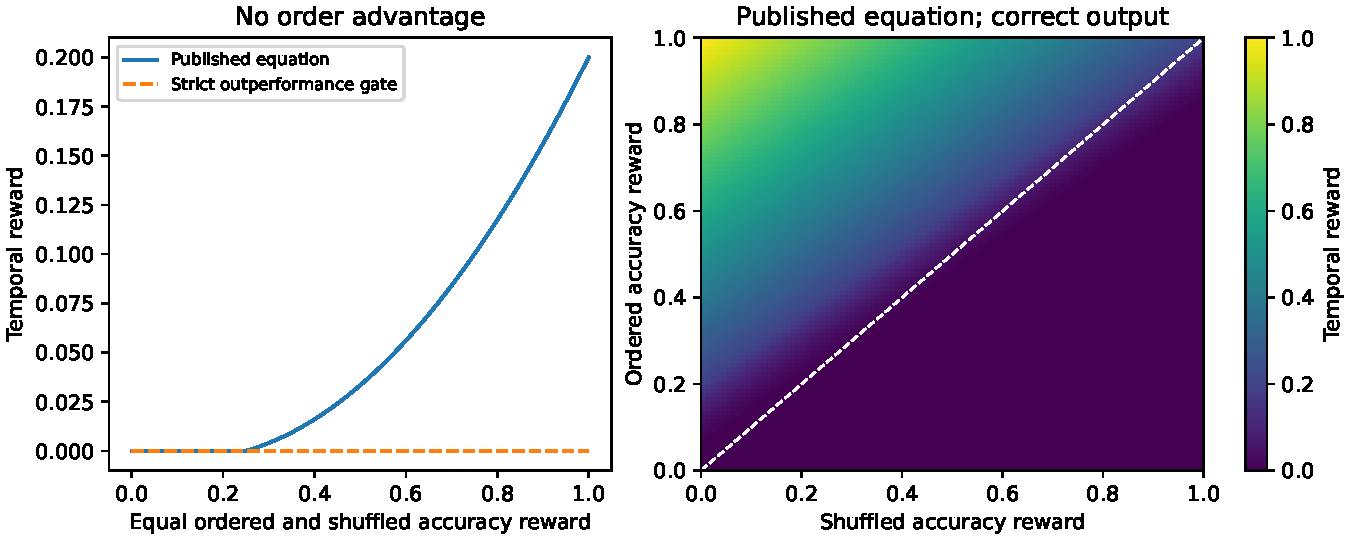
\includegraphics[width=\linewidth]{figures/temporal_reward_audit.pdf}
\caption{Synthetic reward diagnostic. Correct-output assignment assumed. The dashed diagonal marks equal ordered/shuffled accuracy rewards. No GPU inference.}
\end{figure}

\textbf{Next decision:} investigate order-invariant nulls before evidence-question learning. Compare identical-input repeats, fixed permutations, and a separately identified repeated-frame control on original VERA. Previously consulted UCF test data can support exploratory diagnostics, not untouched confirmation or prompt selection. A shuffle response may reflect distribution shift rather than semantic evidence. Check prior diagnostics and implementation code before selecting a GPU pilot.

Instance-Aligned Captions uses manual roles/boxes, SAM2 tracking and VLM-generated captions; these are not wholly human-verified claim labels. Its table includes UCF but not XD. A direct annotation release has not been established from the inspected sources.

\section{Primary sources and review limits}
PrismVAU method sections, LRPO reward/appendix, and the instance-caption annotation pipeline were inspected; several other comparisons currently rely on primary abstracts/introduction and need full-method follow-up. This is not an exhaustive novelty proof.
\begin{itemize}
\item PrismVAU: \url{https://arxiv.org/html/2601.02927v1}
\item ASK-HINT: \url{https://arxiv.org/abs/2510.02155}
\item LRPO: \url{https://proceedings.mlr.press/v306/leng26c.html}
\item GEPA: \url{https://arxiv.org/abs/2507.19457}
\item CCT: \url{https://deepmind.google/research/publications/78755/}
\item Instance-Aligned Captions: \url{https://arxiv.org/html/2601.08155v1}
\end{itemize}
Full decision record, inventory scope and metadata hashes are in studies/vera\_evidence on branch research/vera-evidence-feasibility. No new scientific result or novelty claim is made.
\end{document}
